\section{Resultados}

\subsection{Cobertura da base}

A execução congelada indica que a descoberta nacional é tecnicamente viável, mas que a extração automatizada ainda depende fortemente da qualidade e da estabilidade das instâncias municipais do SAPL. A Figura~\ref{fig:coverage-panel} resume os principais números dessa execução como painel visual de escala, redução e concentração regional.

\begin{figure*}[t]
\centering
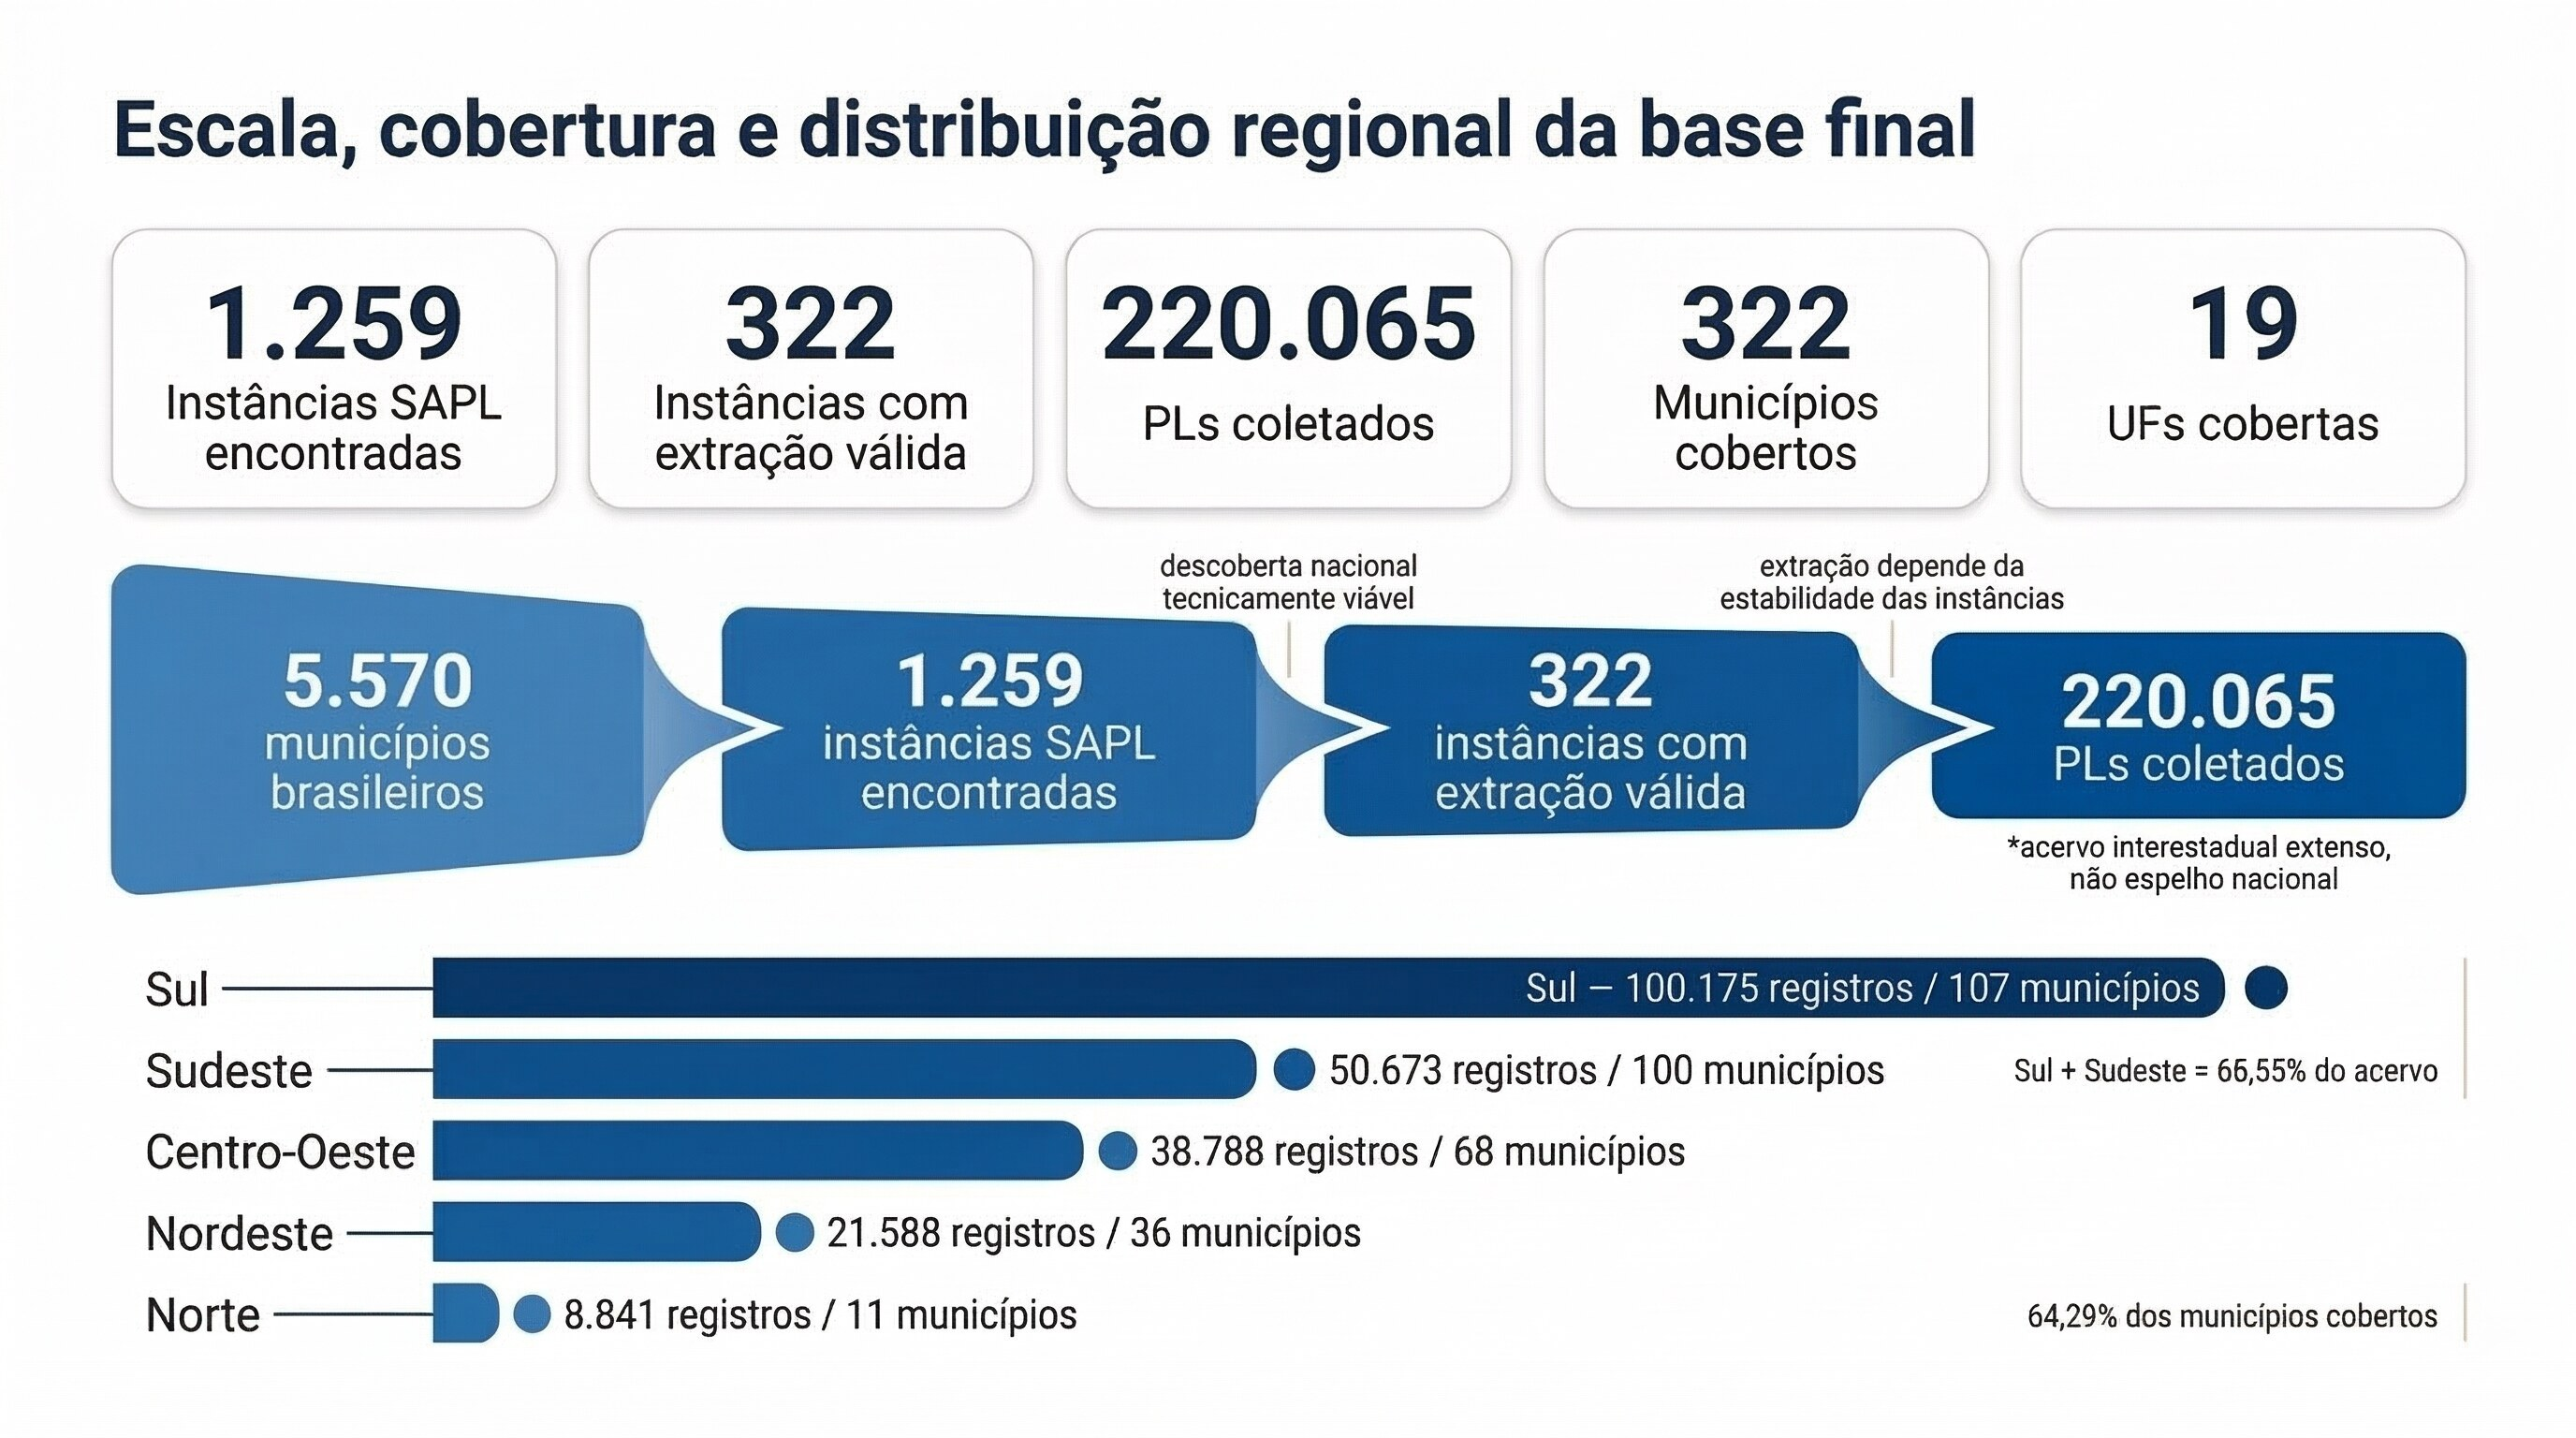
\includegraphics[width=\textwidth]{figures/coverage-panel.jpg}
\caption{Painel visual da execução congelada, combinando indicadores-chave, redução do pipeline e distribuição regional do acervo final.}
\label{fig:coverage-panel}
\end{figure*}

\begin{figure*}[t]
\centering
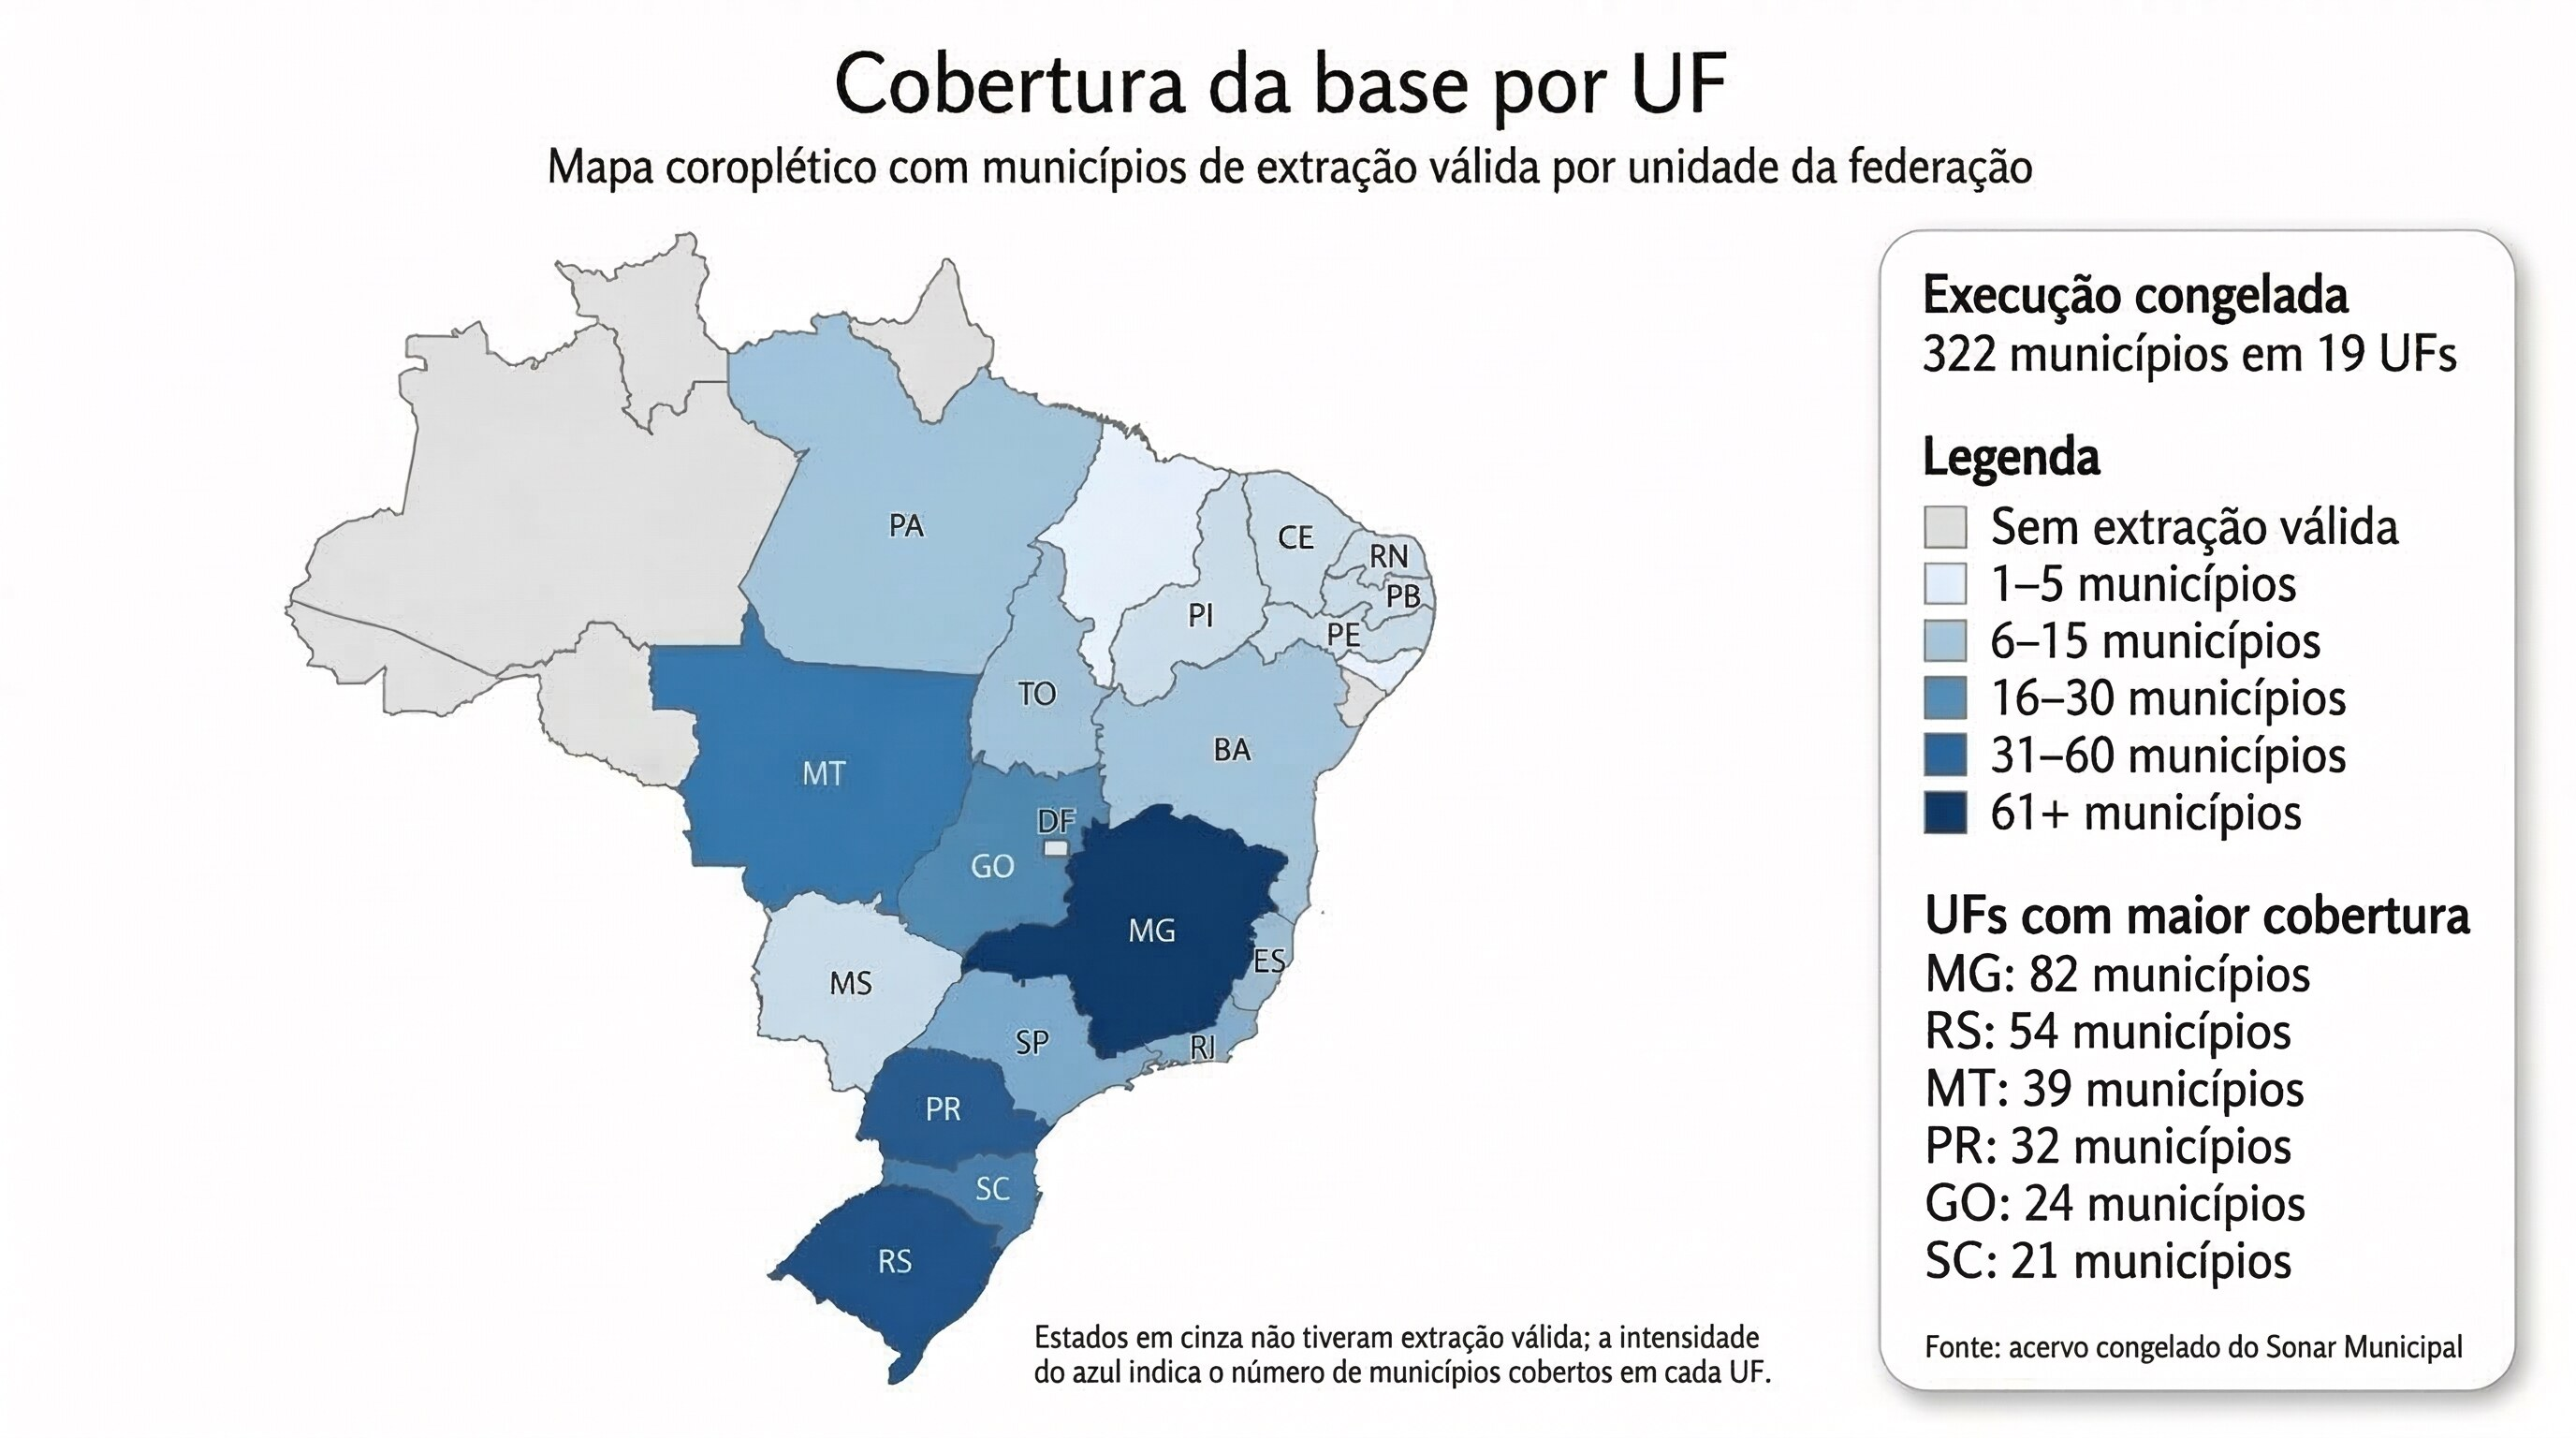
\includegraphics[width=\textwidth]{figures/brazil-coverage-map.jpg}
\caption{Cobertura territorial da base final por UF. Estados em cinza não tiveram extração válida na execução congelada; a intensidade do azul indica o número de municípios cobertos em cada UF.}
\label{fig:brazil-coverage-map}
\end{figure*}

Em termos percentuais, o Sul concentra 45,52\% dos registros e o Sudeste, 23,03\%; juntas, essas duas regiões somam 68,55\% do acervo e 64,29\% dos municípios cobertos. A Figura~\ref{fig:coverage-panel} antecipa essa leitura quantitativa, e a Figura~\ref{fig:brazil-coverage-map} mostra sua distribuição territorial, com cobertura concentrada em 19 UFs e lacunas visíveis em parte do Norte e do Nordeste. O resultado deve ser interpretado como um acervo interestadual extenso, mas não como um espelho nacional da produção legislativa municipal. A base cobre principalmente o período recente da produção legislativa: entre 2021 e 2025, há 96.018 registros distribuídos por 315 municípios. Também foram observados poucos outliers temporais, o que indica necessidade de saneamento antes de análises mais sensíveis ao eixo cronológico.

\subsection{Tradução e busca semântica}

\paragraph{Viabilidade da textualização.}
Na avaliação interna do projeto, o tradutor \textit{ementa} $\rightarrow$ \textit{ação} obteve BERTScore de 84\% no conjunto de validação. A transformação de todo o acervo de 220.065 PLs em ações textualizadas levou 4h47min na execução reportada, o que indica viabilidade operacional nessa escala.

A análise exploratória da base mostrou que a textualização reduz substancialmente o comprimento médio das descrições legislativas sem eliminar a diversidade do acervo. Foram observadas 219.245 ementas únicas e 188.254 ações textualizadas únicas. Em termos práticos, a transformação encurta o texto e reduz variabilidade superficial suficiente para favorecer recuperação semântica e agrupamento; exemplos típicos incluem conversões como ``Institui o Plano Municipal de Saneamento Básico'' para ``Criar plano municipal de saneamento básico''.

\paragraph{Utilidade preliminar da busca.}
A etapa de busca semântica foi avaliada de forma exploratória com consultas reais e julgamento manual preliminar das ações retornadas. Em uma inspeção das cinco consultas públicas de demonstração disponíveis no sistema, 17 dos 25 itens retornados entre os cinco primeiros resultados foram julgados diretamente alinhados ao tema da consulta. Os melhores resultados apareceram em saneamento e evasão escolar, enquanto a consulta sobre arrecadação sem aumento de impostos apresentou o pior desempenho.

Mesmo sem benchmark anotado, a busca produz resultados tematicamente coerentes em consultas substantivas. Para a consulta ``como enfrentar a violência contra a mulher no município?'', por exemplo, a recuperação semântica retornou entre os primeiros itens ações como: regulamentar a violência contra a mulher no município (Uruguaiana/RS), criar política municipal de enfrentamento à violência política contra a mulher (Parauapebas/PA) e promover campanha de denúncia da violência contra a mulher (Anápolis/GO).

\subsection{Estudo de caso: violência contra a mulher}

Entre os temas disponíveis no acervo, violência contra a mulher foi selecionado como estudo de caso principal. O recorte lexical correspondente reúne 2.306 ações distribuídas por 204 municípios e 18 UFs. Esse volume foi considerado adequado para ilustrar o fluxo completo do sistema, desde a consulta em linguagem natural até a consolidação de políticas recorrentes. A Figura~\ref{fig:case-study-flow} sintetiza esse percurso visualmente. Por razões de disponibilidade e cobertura, adotou-se a taxa de homicídios como proxy inicial deste estudo de caso, exclusivamente para fins exploratórios de priorização.

\begin{figure*}[t]
\centering
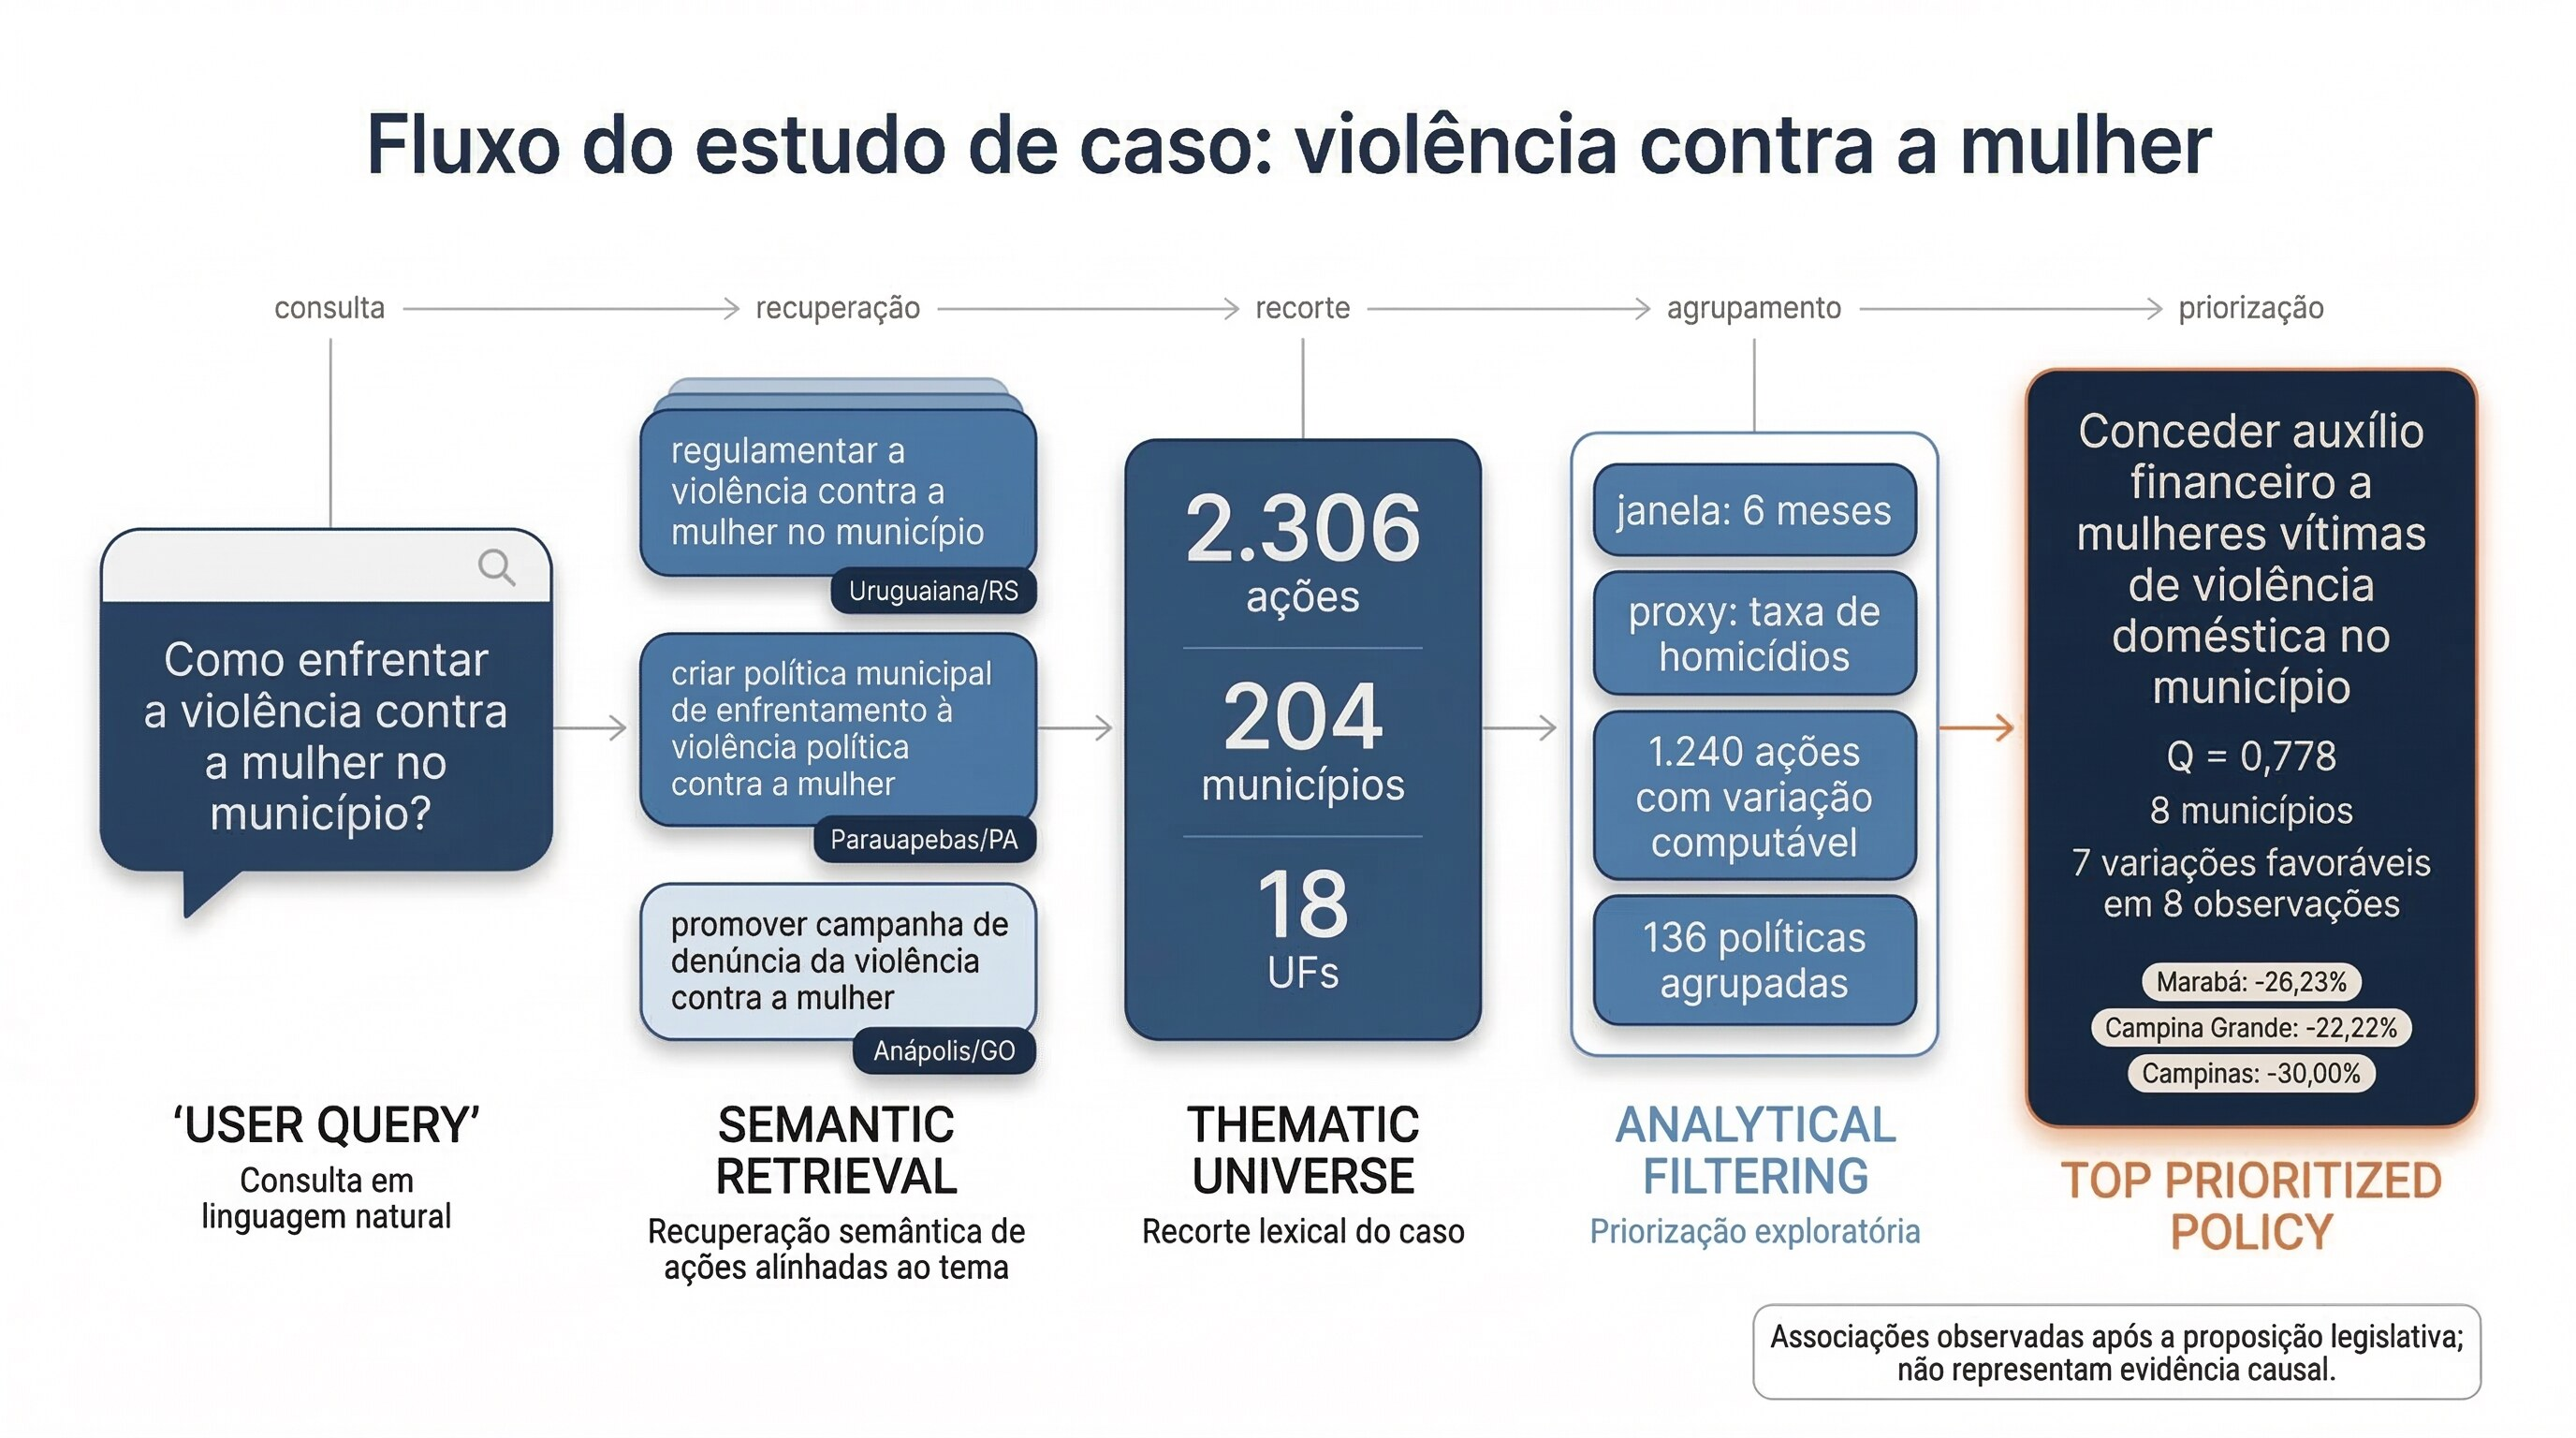
\includegraphics[width=\textwidth]{figures/case-study-flow.jpg}
\caption{Fluxo completo do estudo de caso sobre violência contra a mulher, da consulta em linguagem natural à priorização exploratória de políticas recorrentes.}
\label{fig:case-study-flow}
\end{figure*}

No recorte temático com janela de 6 meses para taxa de homicídios, 1.240 ações tiveram variação computável e geraram 136 políticas agrupadas com pelo menos dois municípios. O cluster com maior escore heurístico foi ``Conceder auxílio financeiro a mulheres vítimas de violência doméstica no município'', com $Q = 0{,}778$, oito municípios representados e sete variações favoráveis em oito observações. Entre os exemplos que compõem esse grupo estão Marabá, Campina Grande e Campinas, com reduções observadas de -26,23\%, -22,22\% e -30,00\%, respectivamente. Esses resultados devem ser interpretados como associações observadas após a proposição legislativa, e não como evidência causal de efetividade.

Além do cluster líder, o estudo de caso indica diversidade de estratégias. Entre os grupos com $Q = 0{,}750$, apareceram propostas de tramitação prioritária para processos envolvendo vítimas de violência doméstica, programas de defesa pessoal para mulheres, programas municipais de enfrentamento ao feminicídio e mecanismos de punição administrativa para autores de violência contra a mulher. Também apareceu um grupo educacional recorrente: ensino de noções básicas sobre a Lei Maria da Penha nas escolas municipais, com oito municípios e $Q = 0{,}667$. A Figura~\ref{fig:case-study-strategies} organiza esse conjunto como mosaico visual de respostas recorrentes.

\begin{figure*}[t]
\centering
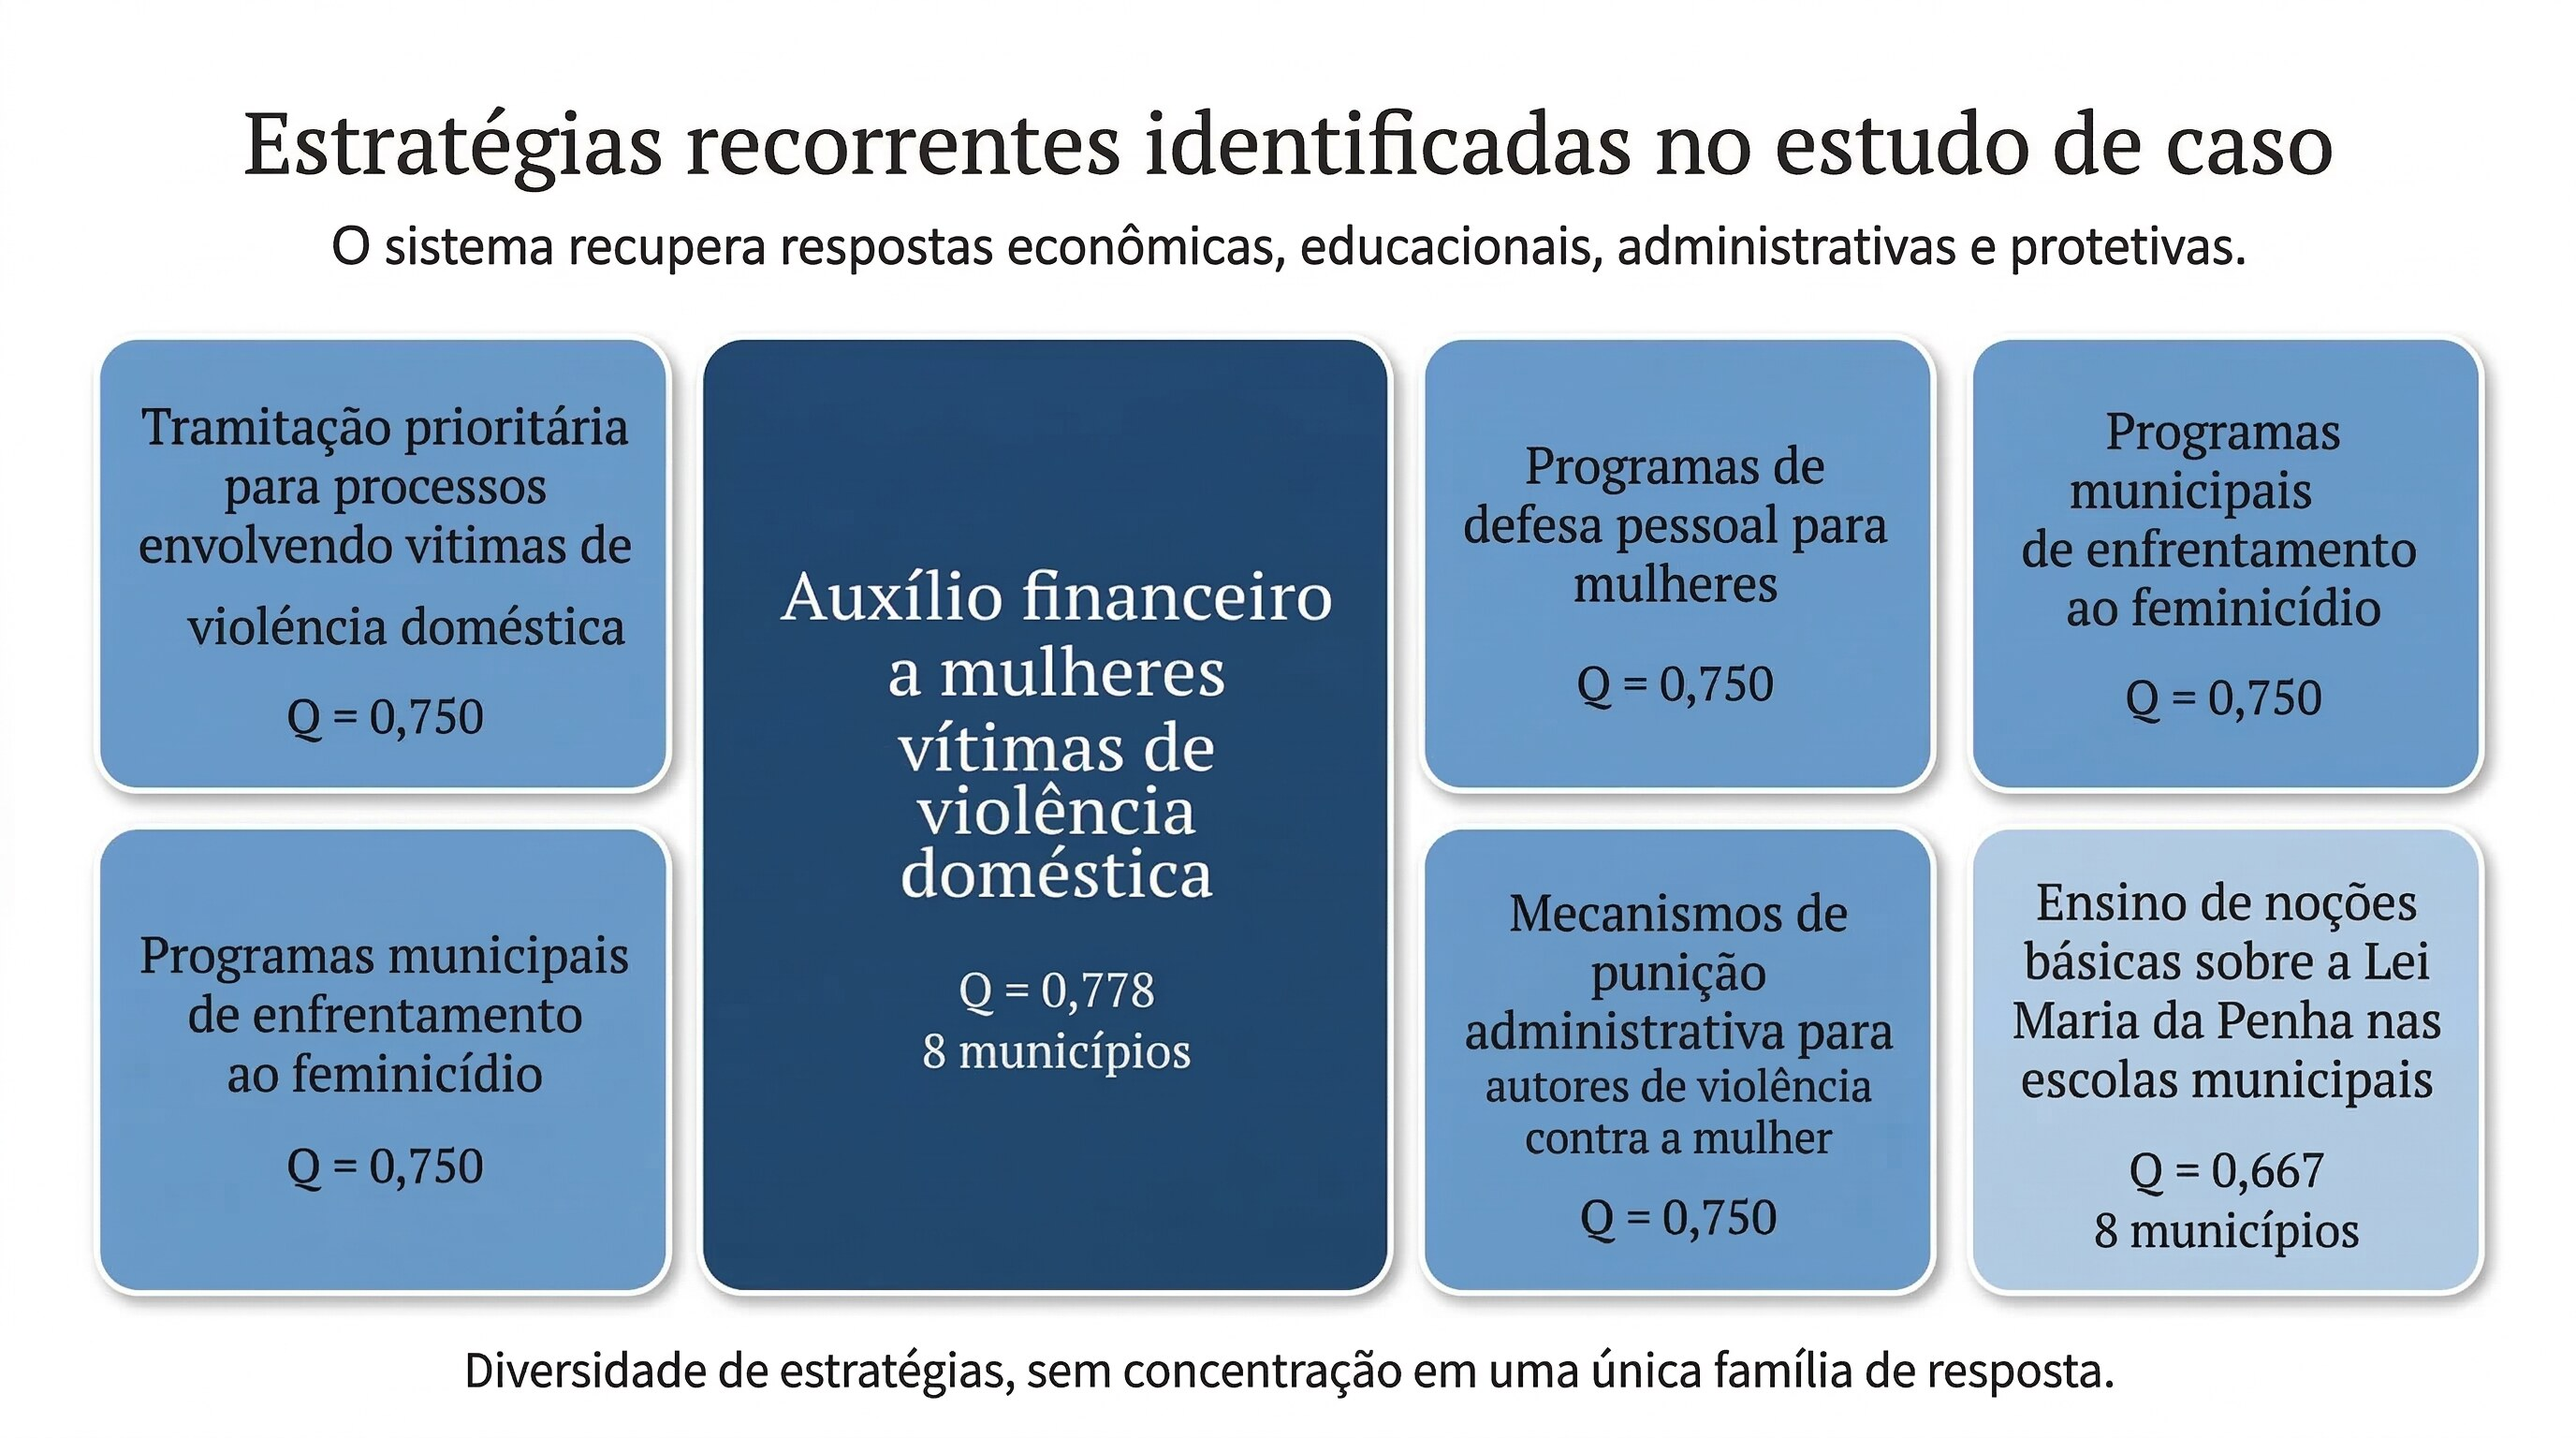
\includegraphics[width=\textwidth]{figures/case-study-strategies.jpg}
\caption{Estratégias recorrentes identificadas no estudo de caso, destacando o cluster líder e a diversidade de respostas econômicas, educacionais, administrativas e protetivas.}
\label{fig:case-study-strategies}
\end{figure*}

\subsection{Falhas observadas}

A inspeção qualitativa apontou dois riscos recorrentes. Na textualização, a condensação pode alterar o sentido material da proposta quando o modelo força uma paráfrase inadequada, como em ``Junho Violeta'' $\rightarrow$ ``Junho Violento''. Nos indicadores, variações de -100\% em janelas futuras com contagem zero podem parecer excessivamente favoráveis em municípios pequenos ou com baixa contagem absoluta de eventos.
